
\documentclass[11pt,a4paper,UTF8]{ctexart}

\usepackage[T1]{fontenc}
\usepackage[utf8]{inputenc}
\usepackage{authblk}

\usepackage{ctex} %导入中文包
\usepackage{tocvsec2}

\usepackage{tabularx}
\usepackage{booktabs} 
\usepackage{multirow}
\usepackage{bbding}
\usepackage{float}

\usepackage{graphicx}
\usepackage{subfigure}

\usepackage{subfiles} %使用多文件方式进行

\usepackage{geometry} %设置页边距的包
\geometry{left=2.5cm,right=2cm,top=2.54cm,bottom=2.54cm} %设置书籍的页边距

\usepackage{hyperref}  %制作pdf的目录
\hypersetup{hidelinks, %去红框
	colorlinks=true,
	allcolors=black,
	pdfstartview=Fit,
	breaklinks=true
}

% 调整itemlist中的行间距
\usepackage{enumitem}
\setenumerate[1]{itemsep=0pt,partopsep=0pt,parsep=\parskip,topsep=5pt}
\setitemize[1]{itemsep=0pt,partopsep=0pt,parsep=\parskip,topsep=5pt}
\setdescription{itemsep=0pt,partopsep=0pt,parsep=\parskip,topsep=5pt}

% 超链接样式设置
\usepackage{hyperref}
\hypersetup{
	colorlinks=true,
	linkcolor=blue,
	filecolor=blue,
	urlcolor=blue,
	citecolor=cyan,
}

\usepackage{indentfirst}

\usepackage{listings}
\usepackage[usenames,dvipsnames,svgnames, x11names]{xcolor}

\usepackage{tcolorbox}

%展示代码
\definecolor{mygreen}{rgb}{0,0.6,0}
\definecolor{mygray}{rgb}{0.5,0.5,0.5}
\definecolor{mymauve}{rgb}{0.58,0,0.82}
\lstset{
	backgroundcolor=\color{blue!3!white}, 
	basicstyle = \footnotesize,       
	breakatwhitespace = false,        
	breaklines = true,                 
	captionpos = b,                    
	commentstyle = \color{mygreen}\bfseries,
	extendedchars = false,             
	frame =shadowbox, 
	framerule=0.5pt,
	keepspaces=true,
	keywordstyle=\color{blue}\bfseries, % keyword style
	language = C++,                     % the language of code
	otherkeywords={string}, 
	numbers=left, 
	numbersep=5pt,
	numberstyle=\tiny\color{mygray},
	rulecolor=\color{black},         
	showspaces=false,  
	showstringspaces=false, 
	showtabs=false,    
	stepnumber=1,         
	stringstyle=\color{mymauve},        % string literal style
	tabsize=2,          
	title=\lstname                      
}

\begin{document}
	%\maketitle
	
	\begin{center}
		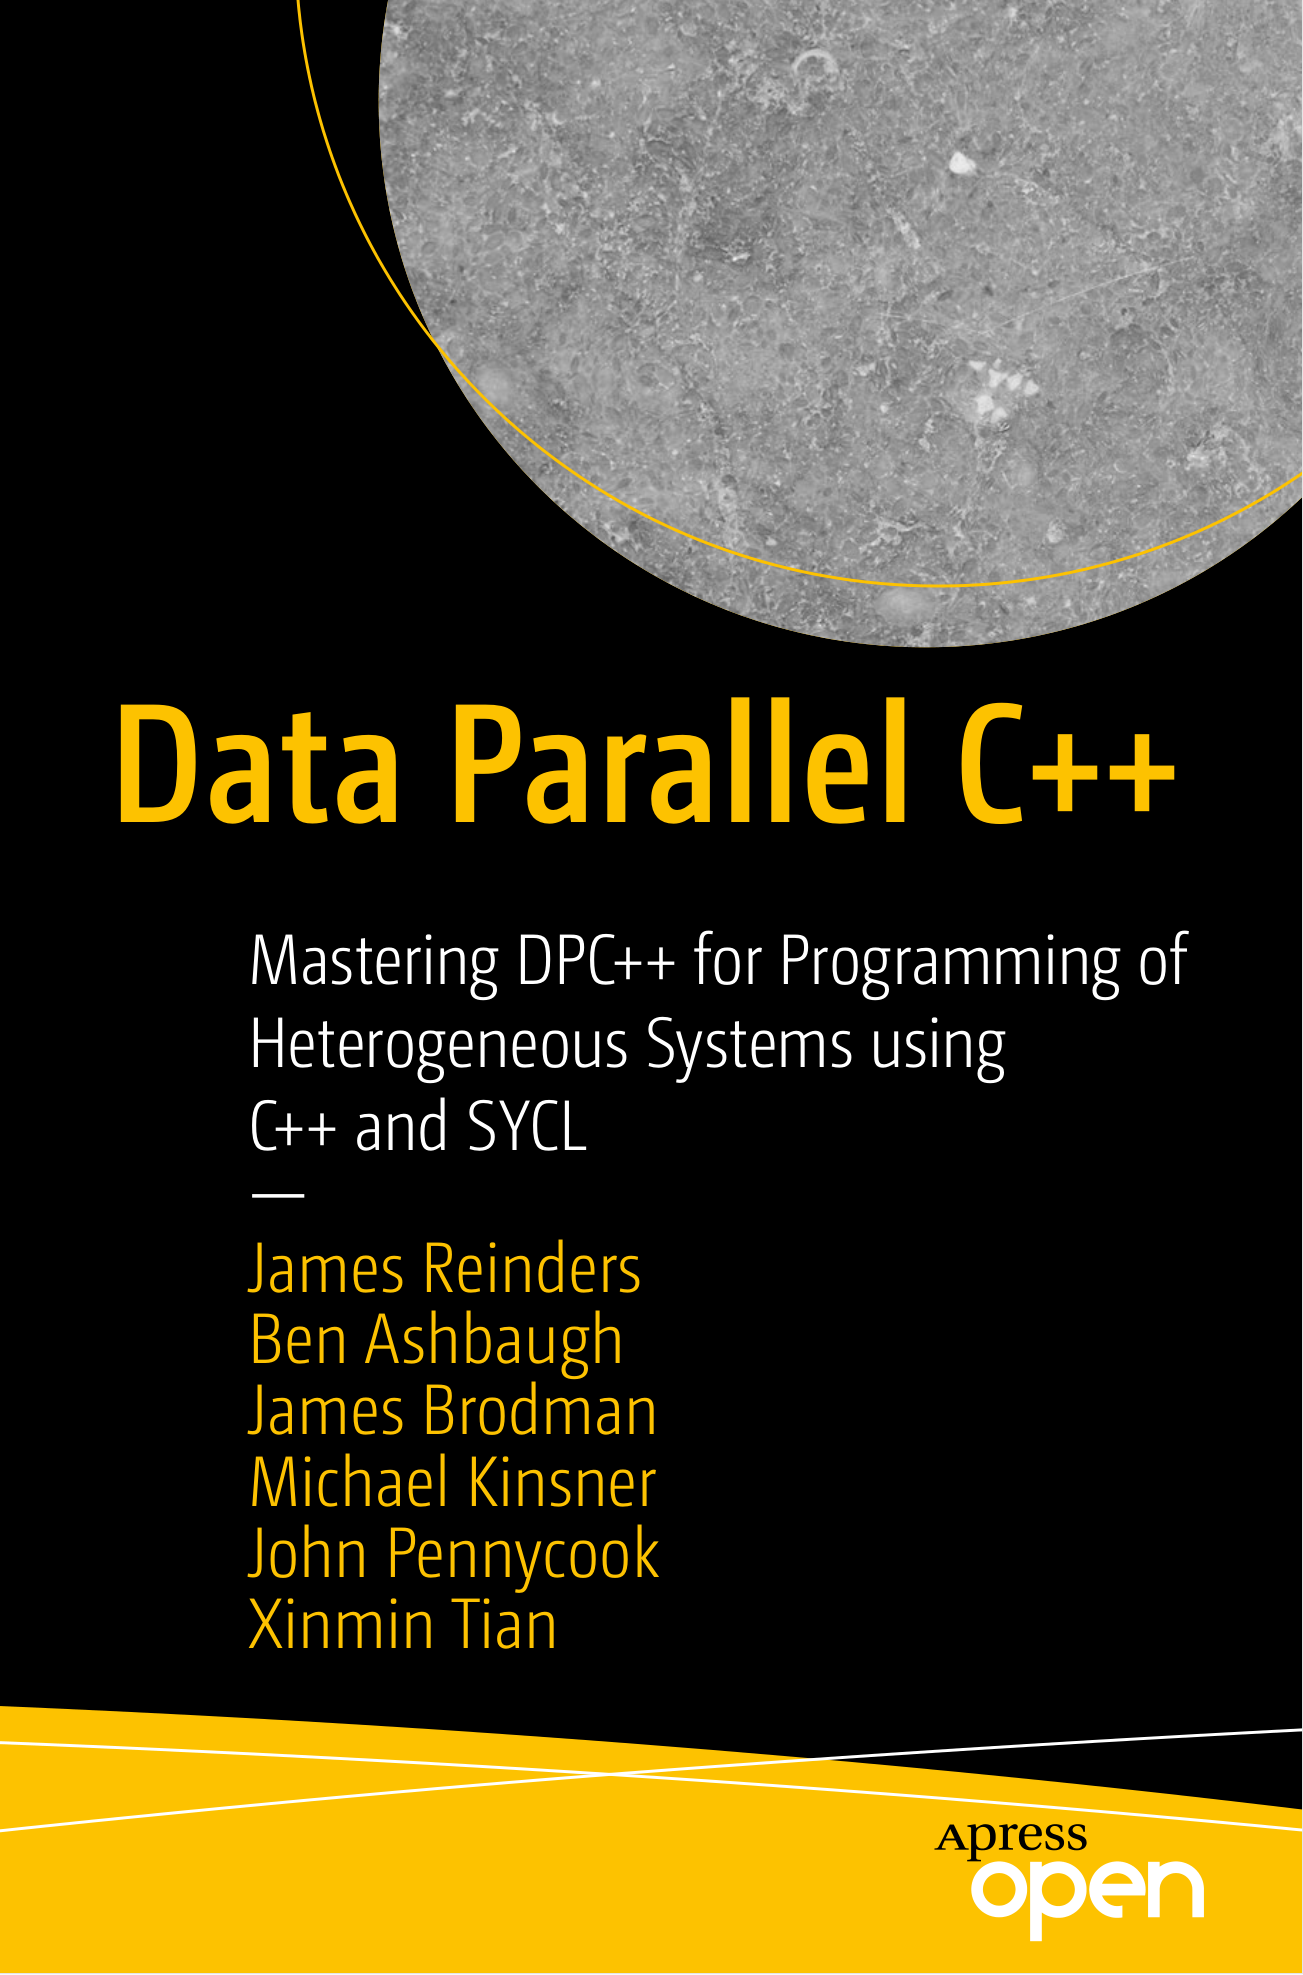
\includegraphics[width=0.9\textwidth]{images/cover}
		\newpage
		\huge
		\textbf{Data Parallel C++} 
		\\[9pt]
		\normalsize
		Mastering DPC++ for Programming of Heterogeneous Systems using C++ and SYCL
		\\[10pt]
		\normalsize 
		作者: James Reinders \&
		Ben Ashbaugh \&
		James Brodman \&
		Michael Kinsner \\
		John Pennycook \&
		Xinmin Tian
		\\[8pt]
		\normalsize
		译者;陈晓伟
	\end{center}
	
	\hspace*{\fill} \\ %插入空行
	\noindent\textbf{本书概述}\ \par
	\begin{center}
		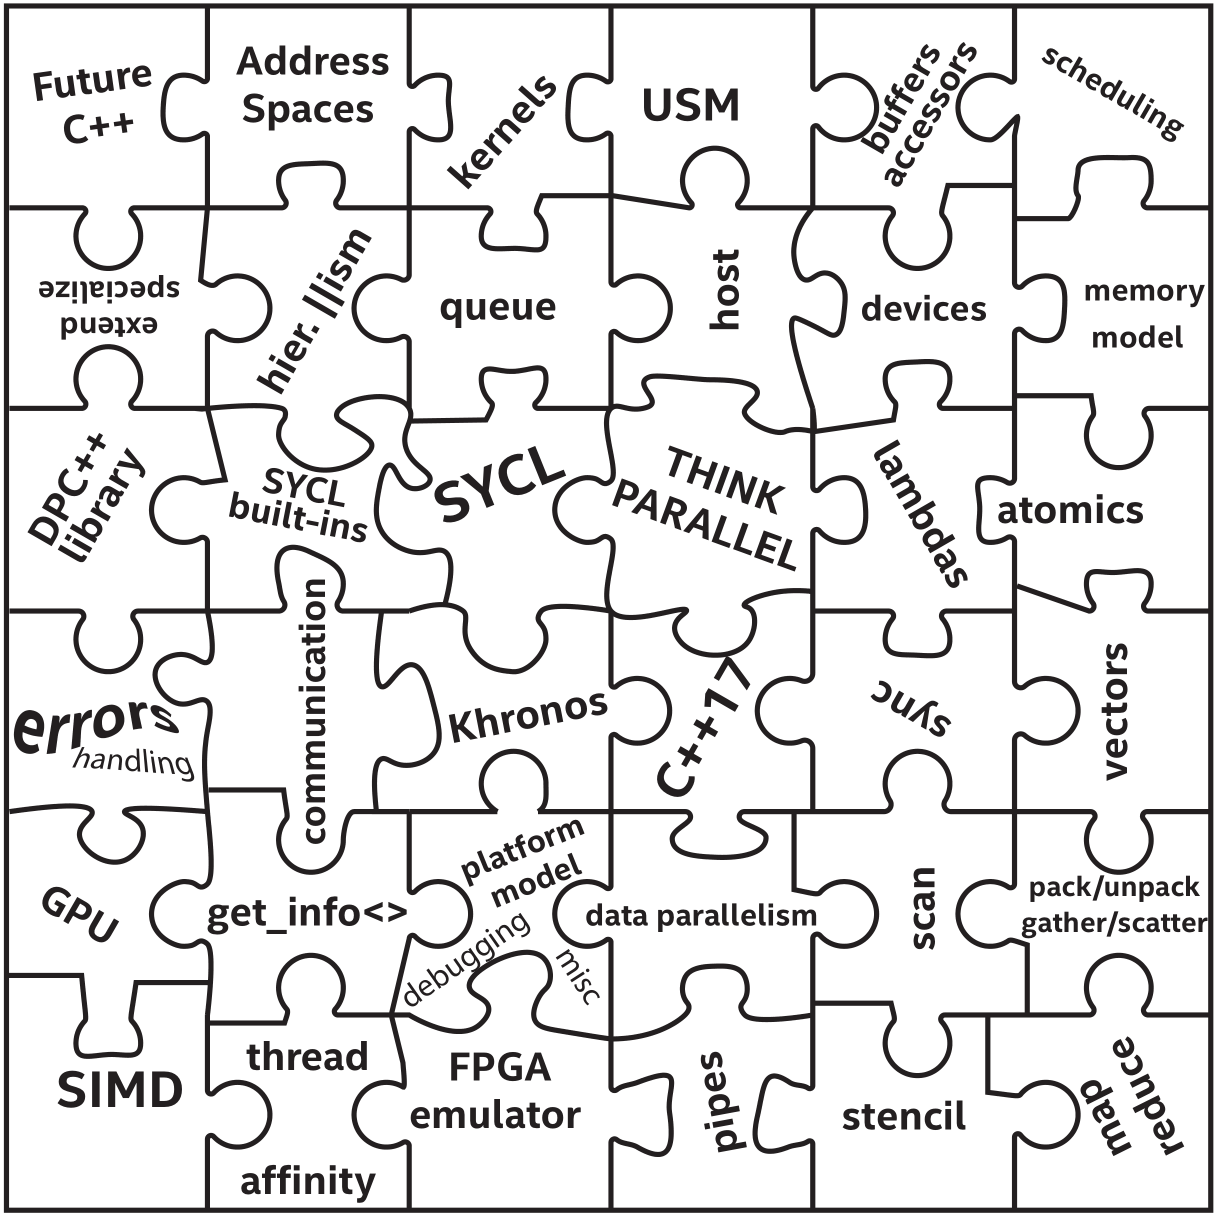
\includegraphics[width=0.5\textwidth]{images/Preface}
	\end{center} \par
	本书是关于使用C++编写数据并行程序的。如果你是并行编程的新手,也没关系。如果从未听说过SYCL或DPC++编译器,也没有关系。\par
	
	SYCL是一个行业驱动的Khronos标准,在异构系统为C++中添加原生的数据并行性。DPC++是一个开源编译器项目,它基于SYCL、编译器扩展和异构支持组成,其中包括GPU、CPU和FPGA支持。本书中的所有例子都是用DPC++编译器编译的。\par
	
	如果你是一个不精通C++的C程序员,不用太担心。本书的几位作者会告诉你,他们是通过阅读使用C++的书籍来学习C++的,就像这本书一样。只要有一点耐心,这本书对于想要编写现代C++程序的C程序员来说应该是很容易的。\par
	
	本书项目始于2019年,对于完全支持C++和数据并行的需要大量的扩展,超出当时的SYCL 1.2.1标准。DPC++编译器需要支持这些扩展,包括对统一共享内存(USM)的支持、通过SYCL完成三级层次结构的子组、匿名lambdas和许多编程简化。\par
	
	本书出版的时候(2020年末),会有一个临时的SYCL 2020规范可供公众评论。临时规范包括对USM、子组、匿名lambdas的支持,以及对编码的简化(类似于C++ 17 CTAD)。可以通过本书中SYCL的扩展,以大致了解SYCL将来的发展方向,这些扩展都会在DPC++编译器项目中实现。我们希望与本书的内容相比,SYCL的变化不会太大,但随着社区的发展,SYCL将会有一些变化。更新信息的重要资源包括本书GitHub和勘误表,可以从本书的网页(www.apress.com/9781484255735)找到,以及oneAPI DPC++参考(tinyurl.com/dpcppref)。\par
	
	SYCL和DPC++的发展仍在继续。在学习了如何使用DPC++为使用SYCL的异构系统创建程序之后,会在之后讨论对未来的展望。\par
	
	希望我们的书能够支持和帮助SYCL社区的发展,并帮助推广C++中的数据并行编程。\par
	
	
	\hspace*{\fill} \\ %插入空行
	\noindent\textbf{作者简介}\ \par
	\textbf{James Reinders}是并行计算领域有30多年经验的专家,参与编纂了十余本与并行编程相关的技术书籍,以及为世界上最快的两台计算机(500强中排名第一)以及许多其他超级计算机和软件开发工具做出了重要贡献。2016年中期结束在Intel的任期(已经在Intel工作了10,001天(超过27年)),不过还继续在并行计算(高性能计算和人工智能)相关的领域进行写作、教学和编程。\par
	
	\textbf{Ben Ashbaugh}是Intel公司的软件架构师,他工作了20多年,为Intel图形产品开发软件驱动程序。在过去的10年里,Ben专注于并行编程模型,用于图形处理器上的通用计算,包括SYCL和DPC++。Ben活跃于Khronos SYCL、OpenCL和SPIR工作组,帮助定义并行编程的行业标准,他编写了许多扩展来展示Intel GPU独特的魅力。\par
	
	\textbf{James Brodman}是Intel公司的软件工程师,专注于并行编程的运行时和编译器开发,并且是DPC++的架构师之一。他拥有伊利诺伊大学厄巴纳-香槟分校的计算机博士学位。\par
	
	\textbf{Michael Kinsner}是Intel公司的首席工程师,为各种架构开发并行编程语言和模型,也是DPC++的架构师之一。他对空间编程模型和编译器做出了重要的贡献,是Khronos组织中的Intel代表,他致力于制定SYCL和OpenCL并行编程行业标准。Mike拥有麦克马斯特大学(McMaster University)的计算机工程博士学位,并且热衷于编写跨架构的编程模型(同时能够保证性能)。\par
	
	\textbf{John Pennycook}是Intel公司的一名HPC应用工程师,专注于让开发人员充分利用现代处理器中的并行性。他在一系列科学领域的应用程序优化和并行方面有丰富的经验,此前曾担任Intel极端性能用户组(IXPUG)指导委员会的代表。John拥有华威大学计算机科学博士学位。他的研究点很多,主要在于跨不同硬件架构实现应用“性能可移植性”的能力。\par
	
	\textbf{Xinmin Tian}是Intel公司高级首席工程师和编译架构师,在OpenMP架构审查委员会(ARB)担任Intel代表。他负责为Intel架构驱动对OpenMP进行装载、向量化和并行化编译器技术。他目前的重点是基于llvm的OpenMP装载,使用oneAPI工具包的DPC++编译器对CPU和Xe加速器进行优化,以及优化HPC/AI应用程序性能。他拥有计算机科学博士学位,拥有27项美国专利,发表了60多篇技术论文,被1200多次引用,并在其专业领域与他人合著了两本书。\par
	
	\hspace*{\fill} \\ %插入空行
	\noindent\textbf{章节架构}\ \par
	\begin{center}
		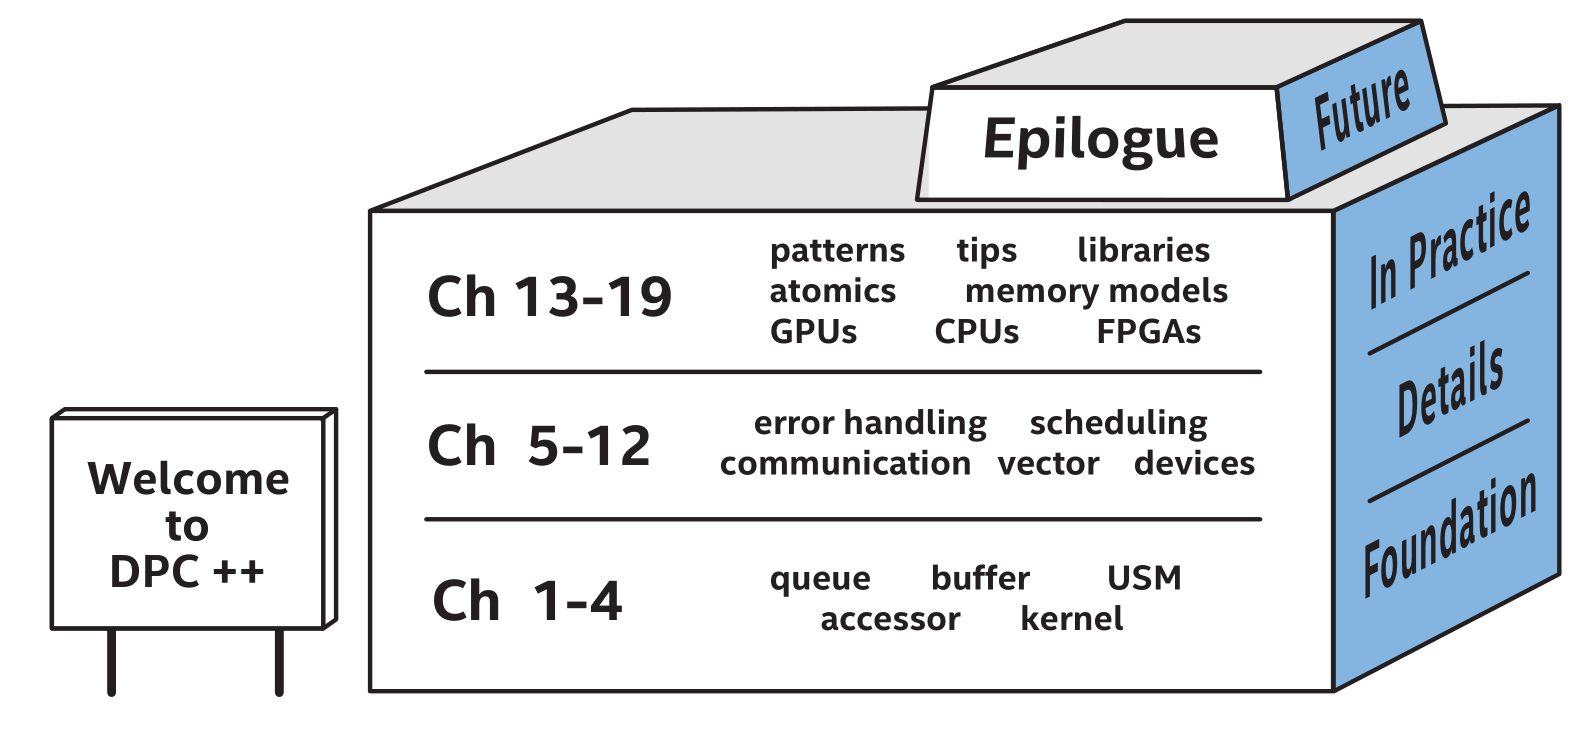
\includegraphics[width=0.5\textwidth]{images/struct-introduce}
	\end{center} \par
	一下子解释一切是很困难的。因此,本书是一个旅程,通过我们需要知道什么,了解如何成为一个高效的数据并行C++开发人员。\par
	
	第1章通过介绍核心概念奠定了基础,这些核心概念要么是新的,要么是需要更新的。\par
	
	第2-4章可以理解为为C++的数据并行编程奠定了基础。读完第1-4章后,我们将为C++中的数据并行编程打下良好的基础。第1-4章是建立在彼此的基础上,最好按顺序阅读。\par
	
	第5-19章在一定程度上相补了一些细节,同时也很容易在需要时进行切换。本书以一个结语结束,讨论了C++数据并行未来可能的方向。\par
	
	希望在学习使用SYCL和DPC++时一切顺利!\par
	
	\hspace*{\fill} \\ %插入空行
	\noindent\textbf{本书相关}\ \par
	\begin{itemize}
		\item github翻译地址:\href{https://github.com/xiaoweiChen/Data-Paralle-Cpp}{https://github.com/xiaoweiChen/Data-Paralle-Cpp}
		\item 英文原版PDF:\href{https://zh.1lib.us/book/6128259/365e5d}{https://zh.1lib.us/book/6128259/365e5d}
		\item 相关教程:\href{https://github.com/jeffhammond/dpcpp-tutorial}{https://github.com/jeffhammond/dpcpp-tutorial}
	\end{itemize}
	\newpage
	
	\tableofcontents
	\newpage
	
	%致谢
	\pagestyle{empty}
	\subfile{content/Acknowledgments.tex}

	\setsecnumdepth{section}
	\section{介绍}
	\subfile{content/chapter-1/1-0.tex}
		\subsection{本书不是说明书}
		\subfile{content/chapter-1/1-1.tex}
		\subsection{SYCL 1.2.1 vs SYCL 2020和DPC++}
		\subfile{content/chapter-1/1-2.tex}
		\subsection{获取DPC++编译器}
		\subfile{content/chapter-1/1-3.tex}
		\subsection{本书代码库}
		\subfile{content/chapter-1/1-4.tex}
		\subsection{Hello, World!SYCL程序解析}
		\subfile{content/chapter-1/1-5.tex}
		\subsection{队列和行动}
		\subfile{content/chapter-1/1-6.tex}
		\subsection{关于并行}
		\subfile{content/chapter-1/1-7.tex}
		\subsection{DPC++和SYCL的关键属性}
		\subfile{content/chapter-1/1-8.tex}
		\subsection{并发和并行}
		\subfile{content/chapter-1/1-9.tex}
		\subsection{总结}
		\subfile{content/chapter-1/1-10.tex}
	\section{代码执行的位置}
	\subfile{content/chapter-2/2-0.tex}
		\subsection{单个源文件}
		\subfile{content/chapter-2/2-1.tex}
		\subsection{选择设备}
		\subfile{content/chapter-2/2-2.tex}
		\subsection{方法1:在任何类型的设备上运行}
		\subfile{content/chapter-2/2-3.tex}
		\subsection{方法2:使用主机设备进行开发和调试}
		\subfile{content/chapter-2/2-4.tex}
		\subsection{方法3:使用GPU(或其他加速器)}
		\subfile{content/chapter-2/2-5.tex}
		\subsection{方法4:使用多个设备}
		\subfile{content/chapter-2/2-6.tex}
		\subsection{方法5:选择自定义(非常具体的)设备}
		\subfile{content/chapter-2/2-7.tex}
		\subsection{在CPU上执行设备端代码的三种方式}
		\subfile{content/chapter-2/2-8.tex}
		\subsection{在设备上创建任务}
		\subfile{content/chapter-2/2-9.tex}
		\subsection{总结}
		\subfile{content/chapter-2/2-10.tex}
	\section{数据管理}
	\subfile{content/chapter-3/3-0.tex}
		\subsection{介绍}
		\subfile{content/chapter-3/3-1.tex}
		\subsection{数据管理的问题}
		\subfile{content/chapter-3/3-2.tex}
		\subsection{本地设备和远程设备}
		\subfile{content/chapter-3/3-4.tex}
		\subsection{管理多种内存}
		\subfile{content/chapter-3/3-5.tex}
		\subsection{统一共享内存、内存和图像}
		\subfile{content/chapter-3/3-6.tex}
		\subsection{统一共享内存}
		\subfile{content/chapter-3/3-7.tex}
		\subsection{内存}
		\subfile{content/chapter-3/3-8.tex}
		\subsection{对数据进行排序}
		\subfile{content/chapter-3/3-9.tex}
		\subsection{选择管理策略}
		\subfile{content/chapter-3/3-10.tex}
		\subsection{句柄类:关键成员}
		\subfile{content/chapter-3/3-11.tex}
		\subsection{总结}
		\subfile{content/chapter-3/3-12.tex}
	\section{并发表示}
	\subfile{content/chapter-4/4-0.tex}
		\subsection{内核间的并行}
		\subfile{content/chapter-4/4-1.tex}
		\subsection{语言的特性}
		\subfile{content/chapter-4/4-2.tex}
		\subsection{内核间的数据并行}
		\subfile{content/chapter-4/4-3.tex}
		\subsection{显式ND-Range内核}
		\subfile{content/chapter-4/4-4.tex}
		\subsection{内核间的分层并行}
		\subfile{content/chapter-4/4-5.tex}
		\subsection{将计算映射到工作项中}
		\subfile{content/chapter-4/4-6.tex}
		\subsection{选择内核形式}
		\subfile{content/chapter-4/4-7.tex}
		\subsection{总结}
		\subfile{content/chapter-4/4-8.tex}
	\section{错误处理}
		\subsection{安全第一}
		\subsection{错误类型}
		\subsection{创建一些错误}
		\subsection{错误的处理策略}
		\subsection{设备上出现错误}
		\subsection{总结}
	\section{统一共享内存}
		\subsection{为什么要使用统一共享内存}
		\subsection{分配类型}
		\subsection{分配内存}
		\subsection{数据管理}
		\subsection{查询}
		\subsection{总结}
	\section{内存}
		\subsection{介绍}
		\subsection{访存}
		\subsection{总结}
	\section{调度内核和数据移动}
		\subsection{什么是图调度?}
		\subsection{图在DPC++中如何工作}
		\subsection{数据传送}
		\subsection{与主机同步}
		\subsection{总结}
	\section{通信和同步}
		\subsection{工作组和工作项}
		\subsection{有效通讯的基础}
		\subsection{使用工作组栅栏和本地内存}
		\subsection{子组}
		\subsection{通用功能}
		\subsection{总结}
	\section{定义内核}
		\subsection{为什么用三种方法来表示内核?}
		\subsection{使用Lambda表达式表示内核}
		\subsection{使用命名的函数对象表示内核}
		\subsection{与其他API的互动性}
		\subsection{程序对象中的内核}
		\subsection{总结}
	\section{向量}
		\subsection{如何使用向量的方式思考}
		\subsection{向量的类型}
		\subsection{向量的接口}
		\subsection{在并行内核中使用向量}
		\subsection{向量并行}
		\subsection{总结}
	\section{设备信息}
		\subsection{优化内核代码}
		\subsection{如何枚举设备和功能}
		\subsection{设备信息描述符}
		\subsection{特定于设备的内核信息描述符}
		\subsection{正确性}
		\subsection{调优/优化}
		\subsection{运行时和编译时属性}
		\subsection{总结}
	\section{实践技巧}
		\subsection{获取DPC++编译器和代码示例}
		\subsection{在线论坛和文档}
		\subsection{平台模型}
		\subsection{将SYCL添加到现有C++代码中}
		\subsection{调试}
		\subsection{初始化数据并访问内核输出}
		\subsection{多个转译单元}
		\subsection{需要为匿名的lambda命名}
		\subsection{将CUDA迁移到SYCL}
		\subsection{总结}
	\section{常见的并行模式}
		\subsection{了解模式}
		\subsection{使用内置函数和库}
		\subsection{直接编程}
		\subsection{总结}
	\section{GPU编程}
		\subsection{性能说明}
		\subsection{GPU的工作原理}
		\subsection{将内核加载到GPU}
		\subsection{GPU内核最佳实践}
		\subsection{总结}
	\section{CPU编程}
		\subsection{性能说明}
		\subsection{通用CPU的基础知识}
		\subsection{SIMD硬件的基础知识}
		\subsection{利用线程级别的并行性}
		\subsection{CPU上的SIMD向量化}
		\subsection{总结}
	\section{FPGA编程}
		\subsection{性能说明}
		\subsection{FPGA的工作原理}
		\subsection{何时使用FPGA}
		\subsection{在FPGA上运行程序}
		\subsection{为FPGA编写内核代码}
		\subsection{一些相关的话题}
		\subsection{总结}
	\section{库}
		\subsection{内置函数}
		\subsection{DPC++库}
		\subsection{总结}
	\section{内存模型和原子操作}
		\subsection{内存模型中有什么?}
		\subsection{内存模型}
		\subsection{实际中的原子操作}
		\subsection{总结}
	\section{结语:DPC++的未来方向}
		\subsection{与C++20和C++23对齐}
		\subsection{地址空间}
		\subsection{扩展与更特化的机制}
		\subsection{分层并行}
		\subsection{总结}
\end{document}